\section{Model of the sensors}

This chapter will, step by step, introduce the sensors, describe how they function and define the methods used to extract the data from them. The accelerometer and gyroscope that we are using are both part of the built-in IMU of the Ardupilot, fitted on 6-axis MPU6000 14-bit chip. The accelerometer works by detecting a force that is actually the opposite of the acceleration vector. This force is not always caused by acceleration, but it can be. It just happens that acceleration causes an inertial force that is captured by the force detection mechanism of the accelerometer. The gyroscope measures the rotation around one of the axes.

\subsubsection{Accelerometer}

To measure the direction of the gravity vector and define the pitch and roll angles, an accelerometer is an easy to use solution.
The raw ADC values obtained from the accelerometer first have to be converted into some acceleration $m/s^2$. To make this happen, a resolution equation is defined that will describe the relationship between the raw values and the acceleration.
For this particular accelerometer, some general acceleration $a_\theta $ along some axis $\theta$ can be found using Equation \ref{sensors1}.

\begin{equation}
\label{sensors1}	
 	a_\theta = \frac{ADC_\theta * g}{bits-1}
\end{equation}

where $ADC_\theta $ is the raw value measured by the sensor, $g$ is the gravitational force and $bits$ is the number of bits the module is running at.
The values measured by the accelerometer will be stored in vector $\bar{a}^B = [\bar{a}_x, \bar{a}_y, \bar{a}_z]^T$. Additionally, these values will be converted into degrees. This process will be discussed in the programming section.

\subsubsection{Gyroscope}

The gyroscope has some similar functionality as the accelerometer, being able to measure the angular velocities expressed as $^{\circ}/s$. The equation to convert raw gyroscope values into angular velocity will be covered in the programming section as well. The measured values of gyroscope will be stored in vector $\bar{\Omega}^B = [\bar{g}_x, \bar{g}_y, \bar{g}]_z^T$.

\section{Programming Accelerometer and Gyroscope}

It is important to understand how the sensors can actually deliver us the data. Usually, they fall into two categories: analogue and digital. The one we are using is digital and it can be programmed using I2C, SPI or USART communication. 

Before getting into the calculations of the angles, we need to get the raw values from both accelerometer and gyroscope and that is done by accessing their registers.

If we want to calculate the inclination of a device relative to the ground for example, we can calculate the angle between the force vector and one of the z-axis. We can do that by manipulating the raw values and by degree conversion. The functions that take care of converting the raw values from both accelerometer and gyroscope are the following:

We have used the Serial Monitor within the Arduino IDE environment to read the outputs from both sensors and they seem to be accurate. The difference in the values of the accelerometer output is because accelerometers are more sensitive to noise and vibrations. The figure below shows the printed outputs at steady state, that is when the quadcopter is parallel to the ground.

We have made separate functions that read from the registers of the accelerometer and gyroscope and that return the raw values of each sensor. These functions are very similar, the only difference being the registers that are accessed to get the information needed. An example of one of the functions is shown Code \ref{c1}.

\lstinputlisting[language=C++, firstline=95, lastline=100, caption={Function that accesses registers and returns a raw value.}, label={code:c1}]{Arduino/acc_gyro_only/acc_gyro_only.ino}

\clearpage

The raw values are then converted into angles by using the functions

\lstinputlisting[language=C++, firstline=144, lastline=163, caption={Function to obtain angles based on the raw values of the accelerometer.}, label={code:c2}]{Arduino/acc_gyro_only/acc_gyro_only.ino}

\lstinputlisting[language=C++, firstline=167, lastline=193, caption={Function to obtain angles based on the raw values of the accelerometer.}, label={code:c3}]{Arduino/acc_gyro_only/acc_gyro_only.ino}

The serial monitor was used to print out the the angles. At steady state, it yielded the results seen in Figure \ref{angles}.

\begin{figure}[H]
  \centering
    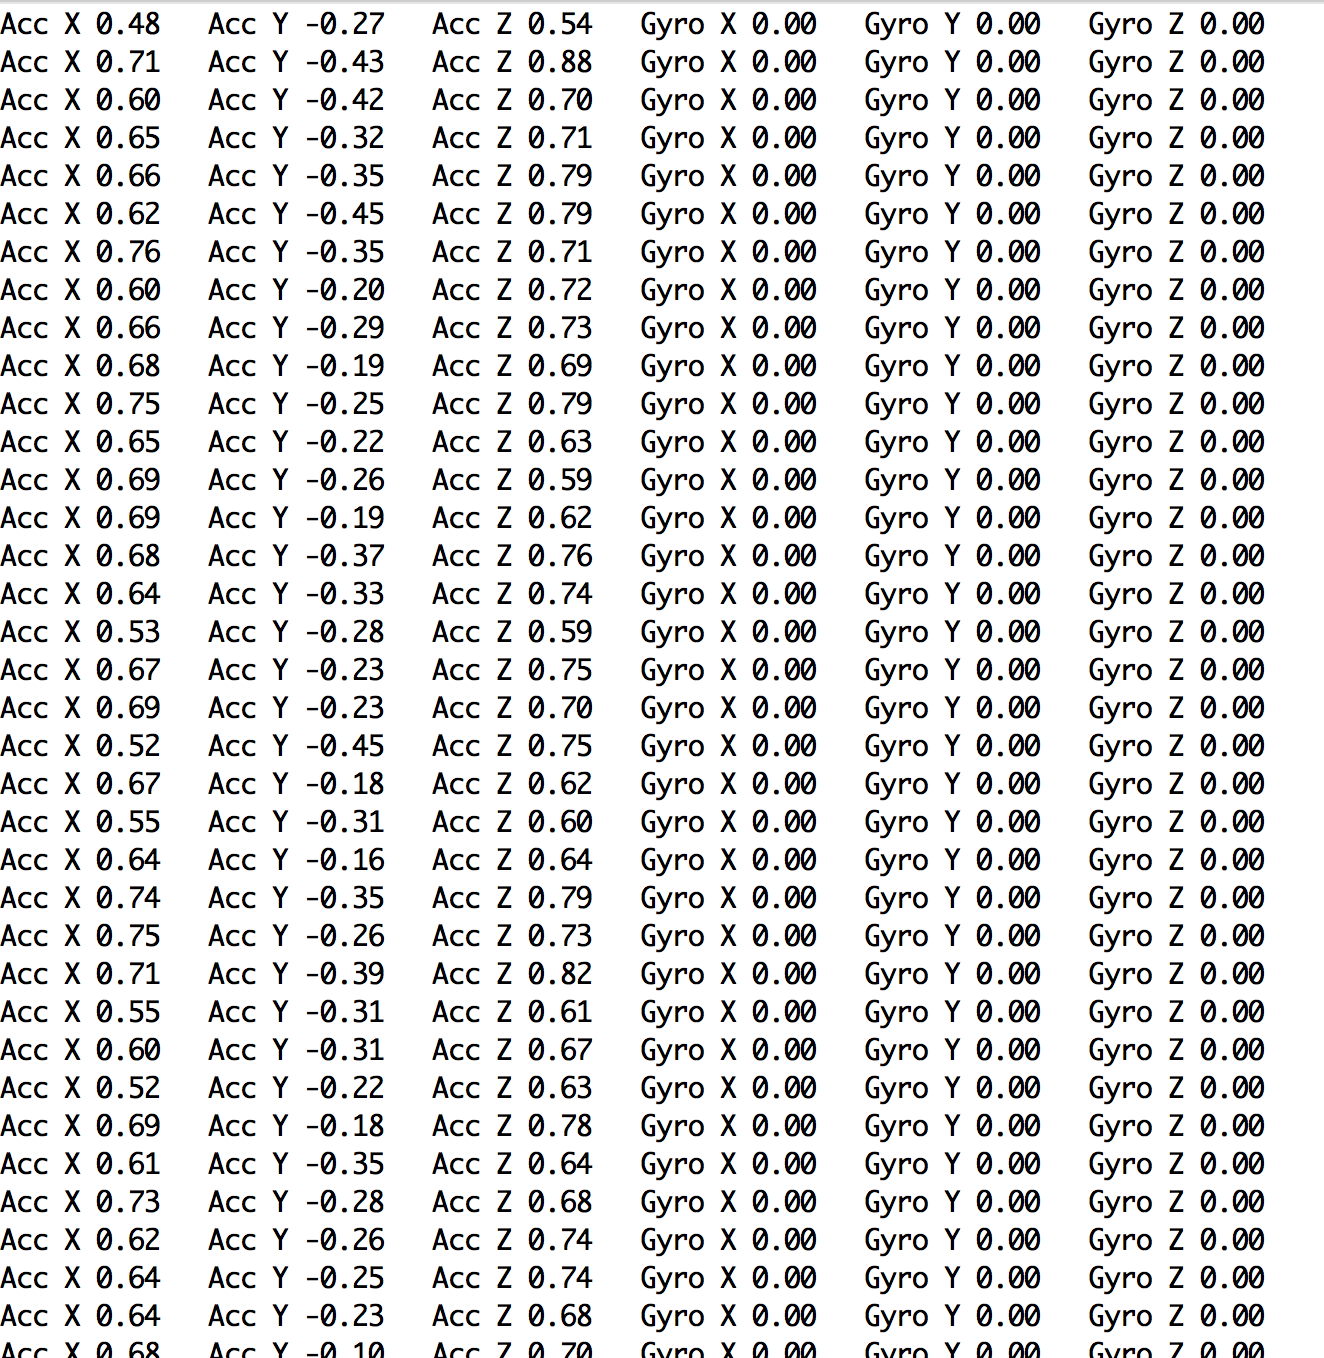
\includegraphics[width=1\textwidth]{images/accgy.png}
	\caption{Angles obtained from Accelerometer and Gyroscope.}
	\label{angles}
\end{figure}

//insert prinscreen for tilting 

\section{Filtering sensor data}
The configuration for the accelerometer and gyroscope enables a low-pass filter at 42Hz. However, looking at the data that the accelerometer reads, there is still some considerable amount of noise and occasional spikes in a steady state. In order to design a filter to counter these problems, flight of the prototype had to be simulated, to record the sensor values when the vehicle goes up in the air and tires to stabilize itself. Therefore, flight controller was unmounted from the frame, connected to a computer and then raised in the air, while tilting it to the sides. The test ran for 30 seconds and provided a $4591\times 6 matrix$, containing 4591 readings for all 3 axis of accelerometer and gyroscope. The plotted data over time for x-axis of the accelerometer and gyroscope can be seen in Figure \ref{dataPlot}.

\begin{figure}[H]
  \centering
    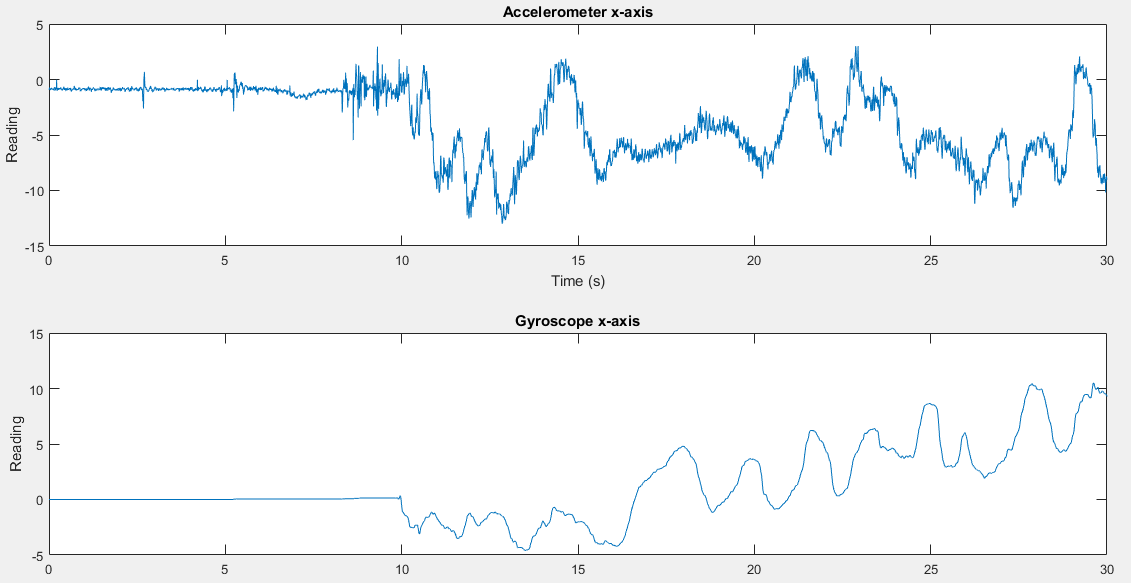
\includegraphics[width=1\textwidth]{images/MPUXPlot.png}
	\caption{Accelerometer and gyroscope x-axis test results.}
	\label{dataPlot}
\end{figure}

The sensor is running at approximately $\frac{4591}{30s} = 153Hz$ frequency, making any additional filter more difficult to perform. However, looking at the test data, it is evident that gyroscope provides clean results just with the help of on-board filter. The main focus then shifts towards the accelerometer - looking at the spectrogram of the accelerometer x-axis data (see Figure \ref{spectrogram}, a low-pass FIR filter is chosen.

\begin{figure}[H]
  \centering
    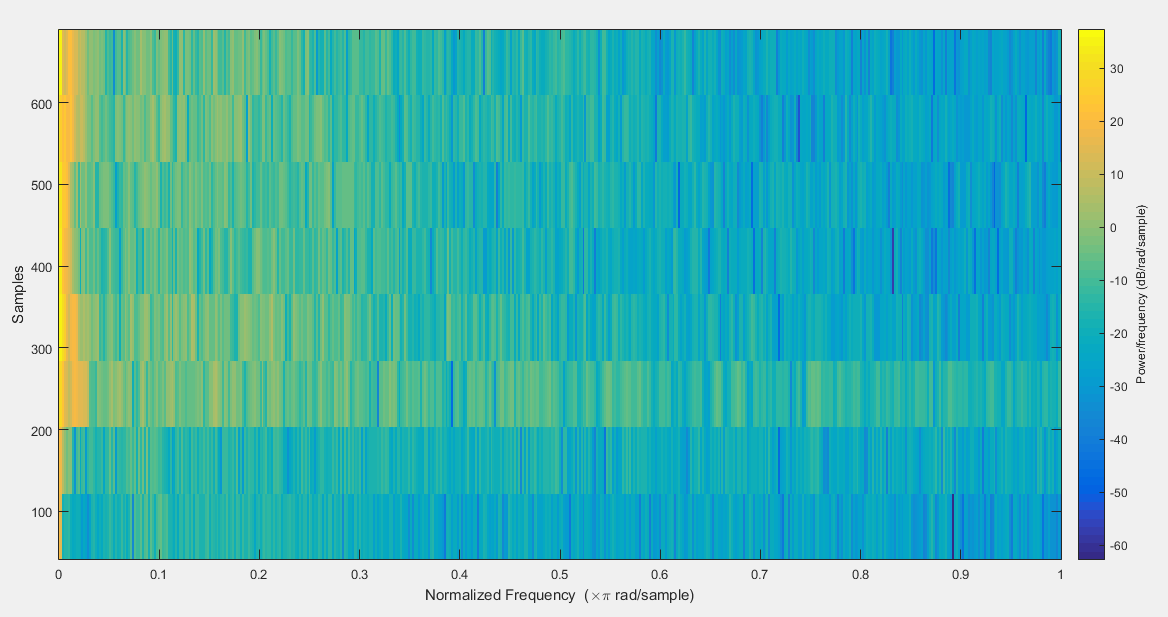
\includegraphics[width=1\textwidth]{images/spectrogram.png}
	\caption{Accelerometer x-axis spectrogram.}
	\label{spectrogram}
\end{figure}

In order to get rid of as much noise as possible, the cut-off frequency was chosen to be the maximum possible value - half of the sampling frequency. The order for the filter was chosen to be 10, mostly through trial and error - at this point, the filter has considerable effect, while not having a very high order, which carries its own cost. The filter was applied to the signal using simple code in Matlab, seen in Listing \ref{code:c4}.

\lstinputlisting[language=Matlab, firstline=1, lastline=6, caption={Filter generation code.}, label={code:c4}]{Arduino/AccelFilter.txt}

The filter was proven to be quite efficient, as seen in Figure \ref{accelFilter}. While not completely perfect, possible improvements will be covered in the discussion chapter.

\begin{figure}[H]
  \centering
    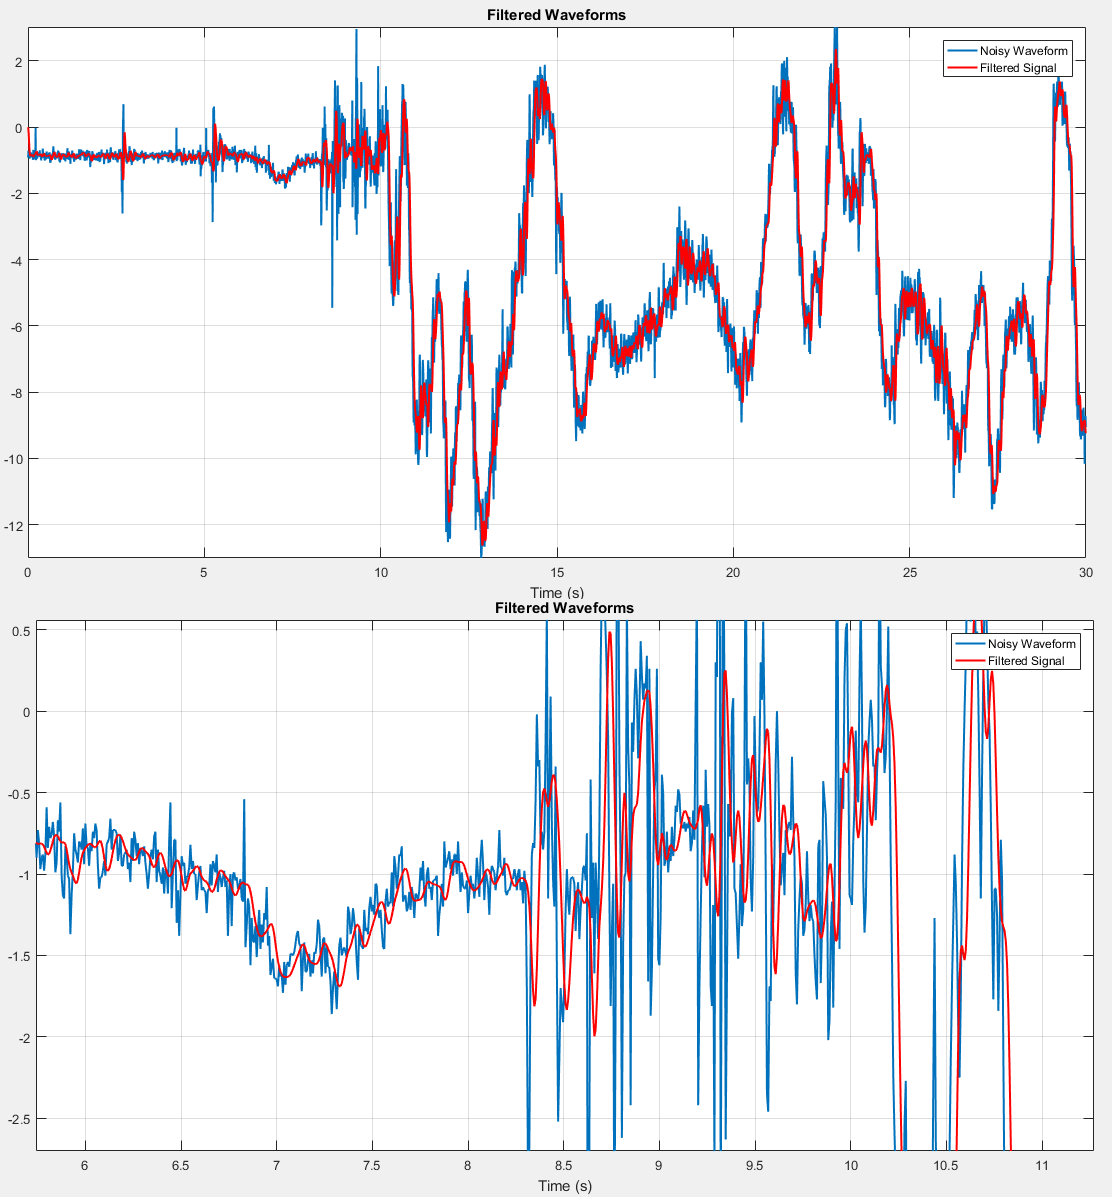
\includegraphics[width=1\textwidth]{images/accelFilter.png}
	\caption{Implemented filter and its close-up.}
	\label{accelFilter}
\end{figure}

%ULTRASONIC NO FILTER <- is it even necessary?